% Statement recovered from Canvas, supplied by Jeremy on 2026-11-02.
% New solution: actual OpenMC runs, data/hw19_results.json; see README.
\begingroup
\raggedbottom
\noindent\textbf{Problem 1}

Use the sodium-cooled fast-reactor unit-cell example from Lesson 19. Let
$x_0$ denote its default fissile-content parameter, using the notebook's
definition and units. Keep geometry, fuel density, coolant, and temperatures
fixed, and run cases with $x=0.5x_0$, $x=x_0$, and $x=1.5x_0$.
Plot $k_\infty$ versus $x$, including the reported uncertainties.
Linearly interpolate between two points that bracket $k_\infty=1$ to
estimate the required fissile content; add a point if needed to obtain a
bracket. Run one calculation at your estimate. Explain the trend using
neutron production and absorption, and explain why this infinite-lattice
threshold is not the critical fissile content of a finite reactor core.

\begin{draftsolution}

\textbf{Definition of fissile content and fixed model.}
The Lesson 19 builder's \texttt{enrichment} argument is the U-235
\emph{atom fraction among uranium atoms}, not a weight percentage and not
an atom fraction among all fuel atoms. The notebook converts its default
15 wt\% U-235 among uranium into
\[
 x_0=\frac{0.15/M_{235}}{0.15/M_{235}+0.85/M_{238}}
 =0.1516279521,
\]
where $M_{235}=235.043928117$ and $M_{238}=238.050786936$ g/mol.
The requested inputs are therefore
\[
 x=0.0758139760,\qquad0.1516279521,\qquad0.2274419281.
\]
These are 7.58140, 15.16280, and 22.74419 atom\% U-235 among uranium.
Multiplying 15 wt\% by the prescribed factors would not give exactly the
same inputs.

Retain the explicit UO$_2$/ODS-steel/sodium regions: fuel radius
$0.4742$ cm, cladding outer radius $0.5419$ cm, nearest-neighbor pitch
$1.1897$ cm, and the notebook's hexagonal prism of height 1 cm.
Fuel, steel, and sodium densities remain 10.5, 7.13, and
$0.837~\mathrm{g/cm^3}$, respectively, at 294 K. The fuel atom ratios are
U-235:U-238:O $=x:(1-x):2$; steel composition is unchanged.
All outer boundaries are reflecting, so the reported eigenvalue represents
$k_\infty$ for this ideal lattice. The notebook's separate illustrative
finite-core target $1/0.90$ is \emph{not} the target requested here.

\textbf{Transport calculations.}
The reference runs use OpenMC 0.16.0, the installed ENDF/B-VIII.0 HDF5
library, 5000 particles per batch, 120 batches, and 30 inactive batches
(one generation per batch). Each case has an independent random seed and
450000 active source histories. Uncertainties below are the reported
one-standard-error Monte Carlo uncertainties, not total modeling or
nuclear-data uncertainties. Exact inputs, seeds, reaction rates, and
source-convergence histories are retained in
\texttt{data/hw19\_results.json}. The saved model builder is
\texttt{hw19\_sfr\_model.py}; the original lesson notebook is unchanged.

% RESULTS_BEGIN
\begin{center}
\begin{tabular}{lrrr}
\hline
Case & U-235 atom\% & $k_\infty\pm s_k$ & Production/absorption \\
\hline
$0.5x_0$ & 7.58140 & $0.934531\pm0.000967$ & 0.93158 \\
$x_0$ & 15.16280 & $1.278583\pm0.000966$ & 1.27248 \\
$1.5x_0$ & 22.74419 & $1.492596\pm0.001126$ & 1.48877 \\
First check & 9.02404 & $1.015286\pm0.000954$ & 1.01240 \\
Refinement 1 & 8.75096 & $0.999839\pm0.000886$ & 0.99788 \\
\hline
\end{tabular}
\end{center}
Production/absorption is the ratio of cell-integrated tally means, not an
independent criticality estimator with a separately propagated uncertainty.
% RESULTS_END

\begin{center}
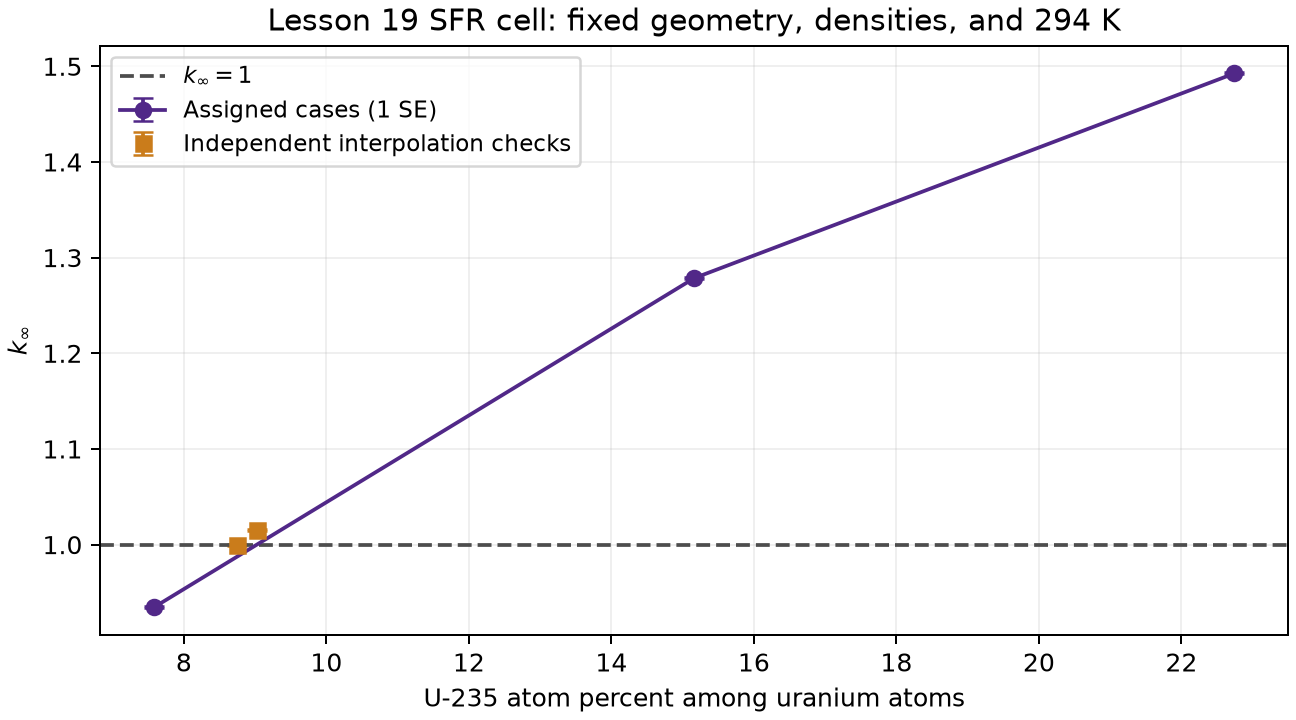
\includegraphics[width=0.94\linewidth]{figures/hw19_enrichment.png}
\end{center}
The error bars are present but small on the full enrichment scale; use the
numerical uncertainties in the table when assessing agreement.

\textbf{Linear interpolation and its limitations.}
For a bracket $(x_L,k_L)$, $(x_H,k_H)$ with $k_L<1<k_H$, use
\[
 \widehat{x}=x_L+(x_H-x_L)\frac{1-k_L}{k_H-k_L}.
\]
The endpoints' independent statistical uncertainties give, to first order,
\[
 s_{\widehat{x}}^2=
 \left[\frac{(x_H-x_L)(1-k_H)}{(k_H-k_L)^2}s_{k_L}\right]^2+
 \left[\frac{(x_H-x_L)(1-k_L)}{(k_H-k_L)^2}s_{k_H}\right]^2.
\]
This uncertainty omits interpolation curvature and systematic model/data
errors. Moreover, later adaptively chosen endpoints can depend on earlier
noisy calculations; treat propagated errors for the refined estimates as
local indicators, not rigorous confidence intervals for the full search.

% INTERPOLATION_BEGIN
The requested $0.5x_0$ and $x_0$ cases already bracket one; no extra
bracketing point is needed. Substitution gives
\[
 \widehat{x}_1=0.090240424,\qquad
 s_{\widehat{x}_1}\simeq 0.0001772,
\]
or $9.02404\pm0.01772$ atom\% from endpoint statistics
alone. The independent calculation at that input gives
\[
 k_\infty(\widehat{x}_1)=1.015286\pm0.000954.
\]
This check is not within two of its reported standard errors of one.
We therefore retain the first result and interpolate again within the
updated local bracket, rather than report the first estimate as an exact root.

Refinement 1 uses the points at
$7.58140$ and
$9.02404$ atom\%, giving
$\widehat{x}_{2}=0.087509595$
(local propagated $s_x\simeq0.0001419$).
Its independent check is $0.999839\pm0.000886$.

The final estimate is approximately
\[
 \boxed{x\simeq 0.087510
 \quad(8.7510\text{ atom\% U-235 among uranium})}.
\]
The final check differs from one by 0.18
of its reported standard errors.

% INTERPOLATION_END

The first bracket and independent run satisfy the assigned procedure;
additional local refinement is an instructor illustration, not an added
student requirement. A student's statistically consistent calculation may
differ from these last digits. An interpolated value need not produce
exactly $k_\infty=1$: both endpoint noise and nonlinearity matter.
Generation estimates and a spatial source-entropy diagnostic are retained
in \texttt{figures/hw19\_convergence.png}; they are useful convergence checks,
not a formal guarantee that the reported variance captures all source
correlation.

\textbf{Why does $k_\infty$ rise?}
Increasing $x$ replaces U-238 with U-235 while preserving UO$_2$
stoichiometry and bulk mass density. In this model the replacement raises
fission-neutron production relative to neutron absorption: more absorptions
can lead to productive fissile fission, rather than non-fission capture in
fertile material. U-238 fast fission still contributes; U-235 also captures,
and steel and sodium absorb. The spectrum and reaction-rate weighting
change with composition, so a globally linear response is not expected.
The cell's volume-integrated \texttt{nu-fission} and \texttt{absorption}
tallies provide a quantitative production/absorption check. Their ratio
should not be forced to equal the eigenvalue exactly: Monte Carlo
estimator differences and non-fission neutron-multiplying reactions can
also enter the neutron balance.

\textbf{Why is this not finite-core critical fissile content?}
The reflecting cell has no neutron leakage. A finite reactor loses
neutrons through its boundary, so in a simplified nonleakage description
\[
 k_{\mathrm{eff}}\simeq P_{\mathrm{NL}}\,k_\infty,
 \qquad P_{\mathrm{NL}}<1.
\]
At the cell threshold $k_\infty=1$, the corresponding leaking system would
have $k_{\mathrm{eff}}<1$. For example, using the notebook's illustrative
$P_{\mathrm{NL}}=0.90$ would instead require $k_\infty\simeq1.1111$;
that is a different question and not a calculated core leakage probability.
Finite-core geometry, reflector, control materials, spatial heterogeneity,
operating temperatures, and composition evolution must be modeled to
estimate actual critical fissile content. This cold, idealized lattice
threshold alone is not such an estimate.

\end{draftsolution}

% Keep display spacing natural before the full-width plot; restore page style.
\clearpage
\endgroup
